\documentclass[a4paper]{article}

%use the english line for english reports
%usepackage[english]{babel}
\usepackage[portuguese]{babel}
\usepackage[utf8]{inputenc}
\usepackage{indentfirst}
\usepackage{graphicx}
\usepackage{verbatim}

\begin{document}
\renewcommand{\figurename}{Fig.}

\setlength{\textwidth}{16cm}
\setlength{\textheight}{22cm}

\title{\Huge\textbf{Título do Trabalho}\linebreak\linebreak\linebreak
\Large\textbf{Relatório Intercalar}\linebreak\linebreak
\linebreak\linebreak

\includegraphics[scale=0.1]{feup-logo.png}\linebreak\linebreak
\linebreak\linebreak
\Large{Mestrado Integrado em Engenharia Informática e Computação} \linebreak\linebreak
\Large{Programação em Lógica}\linebreak
}

\author{\textbf{Grupo Nodes\_3:}\\
Carolina Centeio Jorge - up201403090 \\
Tiago Almeida - up201305665 \\
\linebreak\linebreak \\
 \\ Faculdade de Engenharia da Universidade do Porto \\ Rua Roberto Frias, s\/n, 4200-465 Porto, Portugal \linebreak\linebreak\linebreak
\linebreak\linebreak\vspace{1cm}}

\maketitle
\thispagestyle{empty}

%************************************************************************************************
%************************************************************************************************

\newpage

%Todas as figuras devem ser referidas no texto. %\ref{fig:codigoFigura}
%
%%Exemplo de código para inserção de figuras
%%\begin{figure}[h!]
%%\begin{center}
%%escolher entre uma das seguintes três linhas:
%%\includegraphics[height=20cm,width=15cm]{path relativo da imagem}
%%\includegraphics[scale=0.5]{path relativo da imagem}
%%\includegraphics{path relativo da imagem}
%%\caption{legenda da figura}
%%\label{fig:codigoFigura}
%%\end{center}
%%\end{figure}
%
%
%\textit{Para escrever em itálico}
%\textbf{Para escrever em negrito}
%Para escrever em letra normal
%``Para escrever texto entre aspas''
%
%Para fazer parágrafo, deixar uma linha em branco.
%
%Como fazer bullet points:
%\begin{itemize}
	%\item Item1
	%\item Item2
%\end{itemize}
%
%Como enumerar itens:
%\begin{enumerate}
	%\item Item 1
	%\item Item 2
%\end{enumerate}
%
%\begin{quote}``Isto é uma citação''\end{quote}


%%%%%%%%%%%%%%%%%%%%%%%%%%
\section{Nodes: The Game}

\subsection{History}

Nodes is a board game of abstract strategy, created by The Game Crafter and designed by RGBY Games. It was realeased on September 10, 2016 and it is still on its 1st edition. This game was made for casual gamers, in particular, for people who like chess due to their similarity. Nodes require 2 to 4 players over the age of 12.


\subsection{Brief Description}

\subsubsection{Pieces}

\textbf{Nodes:} Each player starts with \textbf{1} node. Nodes are like kings in chess: they can only move \textbf{one space in each turn}. In this game, they are also communication hubs. They emit signals in all eight directions (front, back, sides and diagonals), called \textbf{lines of communication}.
\newline

\textbf{Units:} Each player starts with \textbf{8} units. Unlike pawns in chess, units can move as many spaces as they want in each turn, \textbf{as long as they are along} a line of communication.

\begin{figure}[h!]
	\centering
	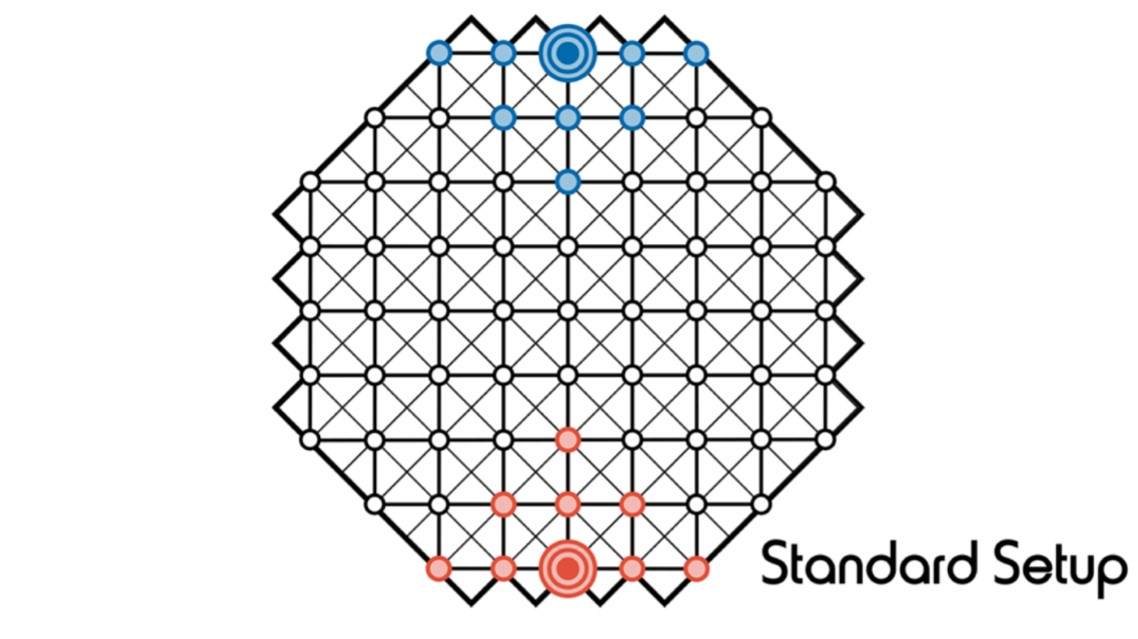
\includegraphics[width=0.5\textwidth]{boardinit.jpg}
	\caption{Initial board set up}
	\label{Image: Initial board set up}
\end{figure}

\subsubsection{Board}
\begin{figure}[!h]

\centering
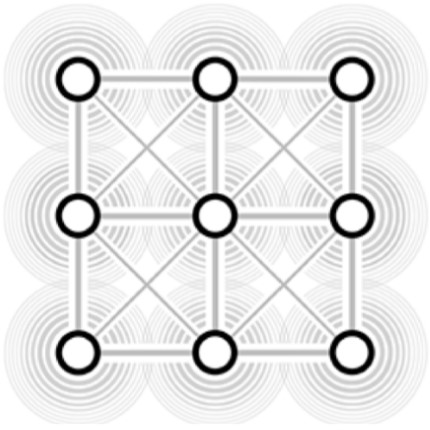
\includegraphics[width=.2\textwidth]{spaces.jpg}
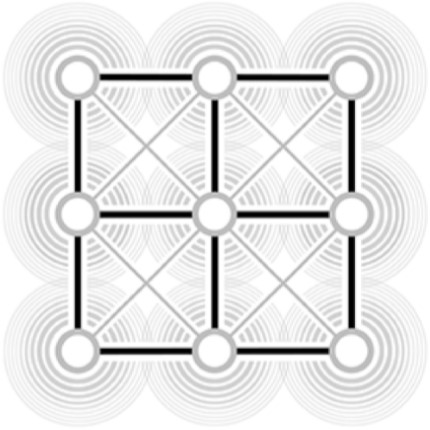
\includegraphics[width=.2\textwidth]{roads.jpg}
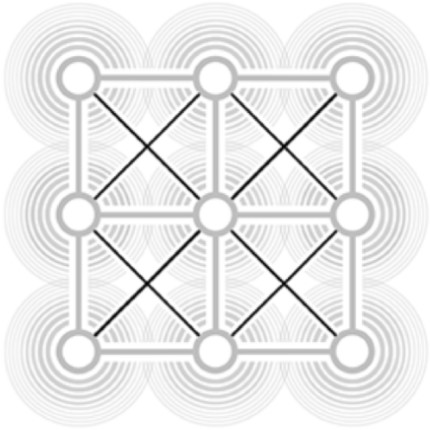
\includegraphics[width=.2\textwidth]{conduits.jpg}

\caption{Spaces, Roads and Conduits}
\label{fig:figure3}

\end{figure}

\textbf{Spaces: }White circles where both units and nodes can finish their turn.

\textbf{Roads: }Boldest lines connecting spaces along which both pieces can draw ther paths.

\textbf{Conduits: }Thin crossing lines that cannot be part of a piece's path.


\subsection{Rules}

\subsubsection{Lines of Communication}

Lines of communication are the basis of the movement. Each node emits a line of communication along each road and conduit that surrounds it. All lines of communication are available in every player's turn, even if they are being emited by another player's node. 


\subsubsection{Unit Movements}

Units can move trough cpmmunication lines util the player decides to finish its turn.
Relay and Interception?



\subsubsection{How to play}



%Descrever detalhadamente o jogo, a sua história e, principalmente, as suas regras.
%Devem ser incluidas imagens apropriadas para explicar o funcionamento do jogo.
%Devem ser incluidas as fontes de informação (e.g. URLs em rodapé).


%%%%%%%%%%%%%%%%%%%%%%%%%%
\section{Representação do Estado do Jogo}

Descrever a forma de representação do estado do tabuleiro (tipicamente uma lista de listas), com exemplificação em Prolog de posições iniciais do jogo, posições intermédias e finais, acompanhadas de imagens ilustrativas.


%%%%%%%%%%%%%%%%%%%%%%%%%%
\section{Visualização do Tabuleiro}

Descrever a forma de visualização do tabuleiro em modo de texto e o(s) predicado(s) Prolog construídos para o efeito.
Deve ser incluída pelo menos uma imagem correspondente ao output produzido pelo predicado de visualização.


%%%%%%%%%%%%%%%%%%%%%%%%%%
\section{Movimentos}

Elencar os movimentos (tipos de jogadas) possíveis e definir os cabeçalhos dos predicados que serão utilizados (ainda não precisam de estar implementados).


\end{document}
